\documentclass[twoside]{book}

% Packages required by doxygen
\usepackage{fixltx2e}
\usepackage{calc}
\usepackage{doxygen}
\usepackage[export]{adjustbox} % also loads graphicx
\usepackage{graphicx}
\usepackage[utf8]{inputenc}
\usepackage{makeidx}
\usepackage{multicol}
\usepackage{multirow}
\PassOptionsToPackage{warn}{textcomp}
\usepackage{textcomp}
\usepackage[nointegrals]{wasysym}
\usepackage[table]{xcolor}

% Font selection
\usepackage[T1]{fontenc}
\usepackage[scaled=.90]{helvet}
\usepackage{courier}
\usepackage{amssymb}
\usepackage{sectsty}
\renewcommand{\familydefault}{\sfdefault}
\allsectionsfont{%
  \fontseries{bc}\selectfont%
  \color{darkgray}%
}
\renewcommand{\DoxyLabelFont}{%
  \fontseries{bc}\selectfont%
  \color{darkgray}%
}
\newcommand{\+}{\discretionary{\mbox{\scriptsize$\hookleftarrow$}}{}{}}

% Page & text layout
\usepackage{geometry}
\geometry{%
  a4paper,%
  top=2.5cm,%
  bottom=2.5cm,%
  left=2.5cm,%
  right=2.5cm%
}
\tolerance=750
\hfuzz=15pt
\hbadness=750
\setlength{\emergencystretch}{15pt}
\setlength{\parindent}{0cm}
\setlength{\parskip}{0.2cm}
\makeatletter
\renewcommand{\paragraph}{%
  \@startsection{paragraph}{4}{0ex}{-1.0ex}{1.0ex}{%
    \normalfont\normalsize\bfseries\SS@parafont%
  }%
}
\renewcommand{\subparagraph}{%
  \@startsection{subparagraph}{5}{0ex}{-1.0ex}{1.0ex}{%
    \normalfont\normalsize\bfseries\SS@subparafont%
  }%
}
\makeatother

% Headers & footers
\usepackage{fancyhdr}
\pagestyle{fancyplain}
\fancyhead[LE]{\fancyplain{}{\bfseries\thepage}}
\fancyhead[CE]{\fancyplain{}{}}
\fancyhead[RE]{\fancyplain{}{\bfseries\leftmark}}
\fancyhead[LO]{\fancyplain{}{\bfseries\rightmark}}
\fancyhead[CO]{\fancyplain{}{}}
\fancyhead[RO]{\fancyplain{}{\bfseries\thepage}}
\fancyfoot[LE]{\fancyplain{}{}}
\fancyfoot[CE]{\fancyplain{}{}}
\fancyfoot[RE]{\fancyplain{}{\bfseries\scriptsize Generated on Wed Jul 15 2015 23\+:08\+:05 for Login\+Scrape by Doxygen }}
\fancyfoot[LO]{\fancyplain{}{\bfseries\scriptsize Generated on Wed Jul 15 2015 23\+:08\+:05 for Login\+Scrape by Doxygen }}
\fancyfoot[CO]{\fancyplain{}{}}
\fancyfoot[RO]{\fancyplain{}{}}
\renewcommand{\footrulewidth}{0.4pt}
\renewcommand{\chaptermark}[1]{%
  \markboth{#1}{}%
}
\renewcommand{\sectionmark}[1]{%
  \markright{\thesection\ #1}%
}

% Indices & bibliography
\usepackage{natbib}
\usepackage[titles]{tocloft}
\setcounter{tocdepth}{3}
\setcounter{secnumdepth}{5}
\makeindex

% Hyperlinks (required, but should be loaded last)
\usepackage{ifpdf}
\ifpdf
  \usepackage[pdftex,pagebackref=true]{hyperref}
\else
  \usepackage[ps2pdf,pagebackref=true]{hyperref}
\fi
\hypersetup{%
  colorlinks=true,%
  linkcolor=blue,%
  citecolor=blue,%
  unicode%
}

% Custom commands
\newcommand{\clearemptydoublepage}{%
  \newpage{\pagestyle{empty}\cleardoublepage}%
}


%===== C O N T E N T S =====

\begin{document}

% Titlepage & ToC
\hypersetup{pageanchor=false,
             bookmarks=true,
             bookmarksnumbered=true,
             pdfencoding=unicode
            }
\pagenumbering{roman}
\begin{titlepage}
\vspace*{7cm}
\begin{center}%
{\Large Login\+Scrape }\\
\vspace*{1cm}
{\large Generated by Doxygen 1.8.10}\\
\vspace*{0.5cm}
{\small Wed Jul 15 2015 23:08:05}\\
\end{center}
\end{titlepage}
\clearemptydoublepage
\tableofcontents
\clearemptydoublepage
\pagenumbering{arabic}
\hypersetup{pageanchor=true}

%--- Begin generated contents ---
\chapter{Namespace Index}
\section{Packages}
Here are the packages with brief descriptions (if available)\+:\begin{DoxyCompactList}
\item\contentsline{section}{\hyperlink{namespace_login_scrape}{Login\+Scrape} }{\pageref{namespace_login_scrape}}{}
\end{DoxyCompactList}

\chapter{Hierarchical Index}
\section{Class Hierarchy}
This inheritance list is sorted roughly, but not completely, alphabetically\+:\begin{DoxyCompactList}
\item Form\begin{DoxyCompactList}
\item \contentsline{section}{Login\+Scrape.\+Form1}{\pageref{class_login_scrape_1_1_form1}}{}
\item \contentsline{section}{Login\+Scrape.\+Login}{\pageref{class_login_scrape_1_1_login}}{}
\end{DoxyCompactList}
\item \contentsline{section}{Login\+Scrape.\+Scraper}{\pageref{class_login_scrape_1_1_scraper}}{}
\begin{DoxyCompactList}
\item \contentsline{section}{Login\+Scrape.\+Reddit\+Karma\+Scraper}{\pageref{class_login_scrape_1_1_reddit_karma_scraper}}{}
\end{DoxyCompactList}
\end{DoxyCompactList}

\chapter{Class Index}
\section{Class List}
Here are the classes, structs, unions and interfaces with brief descriptions\+:\begin{DoxyCompactList}
\item\contentsline{section}{\hyperlink{class_login_scrape_1_1_form1}{Login\+Scrape.\+Form1} }{\pageref{class_login_scrape_1_1_form1}}{}
\item\contentsline{section}{\hyperlink{class_login_scrape_1_1_login}{Login\+Scrape.\+Login} }{\pageref{class_login_scrape_1_1_login}}{}
\item\contentsline{section}{\hyperlink{class_login_scrape_1_1_reddit_karma_scraper}{Login\+Scrape.\+Reddit\+Karma\+Scraper} }{\pageref{class_login_scrape_1_1_reddit_karma_scraper}}{}
\item\contentsline{section}{\hyperlink{class_login_scrape_1_1_scraper}{Login\+Scrape.\+Scraper} }{\pageref{class_login_scrape_1_1_scraper}}{}
\end{DoxyCompactList}

\chapter{Namespace Documentation}
\hypertarget{namespace_login_scrape}{}\section{Login\+Scrape Namespace Reference}
\label{namespace_login_scrape}\index{Login\+Scrape@{Login\+Scrape}}
\subsection*{Classes}
\begin{DoxyCompactItemize}
\item 
class \hyperlink{class_login_scrape_1_1_form1}{Form1}
\item 
class \hyperlink{class_login_scrape_1_1_login}{Login}
\item 
class {\bfseries Program}
\item 
class \hyperlink{class_login_scrape_1_1_reddit_karma_scraper}{Reddit\+Karma\+Scraper}
\item 
class \hyperlink{class_login_scrape_1_1_scraper}{Scraper}
\end{DoxyCompactItemize}
\subsection*{Enumerations}
\begin{DoxyCompactItemize}
\item 
\hypertarget{namespace_login_scrape_a5a49771eff6d809d7c335f178ab22286}{}enum {\bfseries Scraper\+State} \{ {\bfseries L\+O\+G\+I\+N}, 
{\bfseries F\+R\+O\+N\+T\+\_\+\+P\+A\+G\+E}
 \}\label{namespace_login_scrape_a5a49771eff6d809d7c335f178ab22286}

\end{DoxyCompactItemize}

\chapter{Class Documentation}
\hypertarget{class_login_scrape_1_1_form1}{}\section{Login\+Scrape.\+Form1 Class Reference}
\label{class_login_scrape_1_1_form1}\index{Login\+Scrape.\+Form1@{Login\+Scrape.\+Form1}}
Inheritance diagram for Login\+Scrape.\+Form1\+:\begin{figure}[H]
\begin{center}
\leavevmode
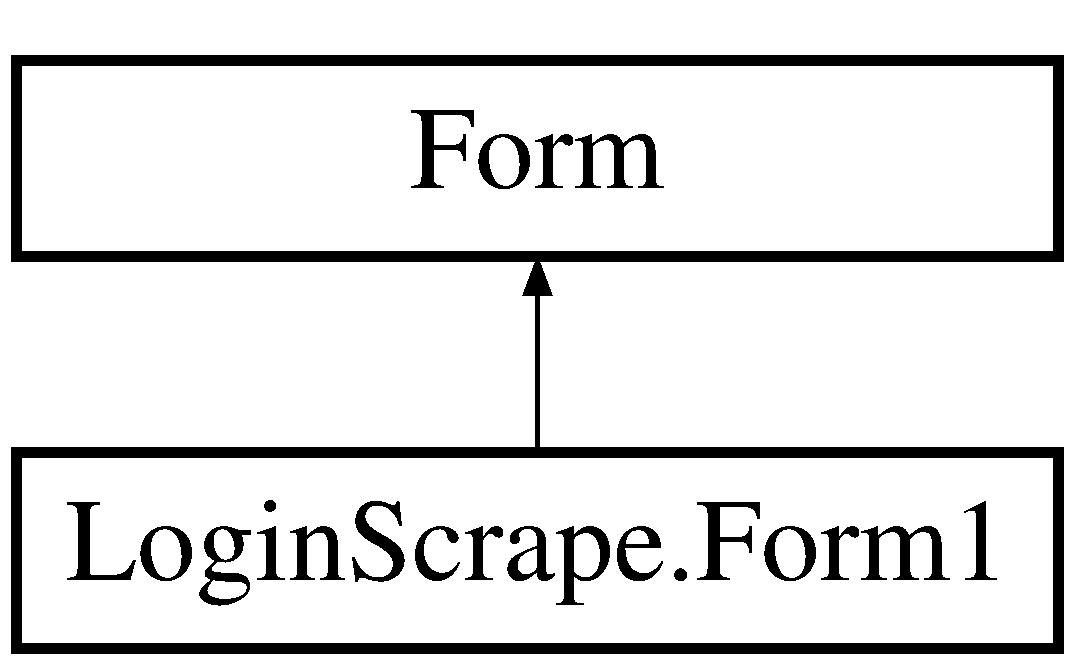
\includegraphics[height=2.000000cm]{class_login_scrape_1_1_form1}
\end{center}
\end{figure}
\subsection*{Protected Member Functions}
\begin{DoxyCompactItemize}
\item 
override void \hyperlink{class_login_scrape_1_1_form1_a97e5c97173afac90d064c5f4670a0e73}{Dispose} (bool disposing)
\begin{DoxyCompactList}\small\item\em Clean up any resources being used. \end{DoxyCompactList}\end{DoxyCompactItemize}


\subsection{Member Function Documentation}
\hypertarget{class_login_scrape_1_1_form1_a97e5c97173afac90d064c5f4670a0e73}{}\index{Login\+Scrape\+::\+Form1@{Login\+Scrape\+::\+Form1}!Dispose@{Dispose}}
\index{Dispose@{Dispose}!Login\+Scrape\+::\+Form1@{Login\+Scrape\+::\+Form1}}
\subsubsection[{Dispose(bool disposing)}]{\setlength{\rightskip}{0pt plus 5cm}override void Login\+Scrape.\+Form1.\+Dispose (
\begin{DoxyParamCaption}
\item[{bool}]{disposing}
\end{DoxyParamCaption}
)\hspace{0.3cm}{\ttfamily [protected]}}\label{class_login_scrape_1_1_form1_a97e5c97173afac90d064c5f4670a0e73}


Clean up any resources being used. 


\begin{DoxyParams}{Parameters}
{\em disposing} & true if managed resources should be disposed; otherwise, false.\\
\hline
\end{DoxyParams}


The documentation for this class was generated from the following files\+:\begin{DoxyCompactItemize}
\item 
Form1.\+cs\item 
Form1.\+Designer.\+cs\end{DoxyCompactItemize}

\hypertarget{class_login_scrape_1_1_login}{}\section{Login\+Scrape.\+Login Class Reference}
\label{class_login_scrape_1_1_login}\index{Login\+Scrape.\+Login@{Login\+Scrape.\+Login}}
Inheritance diagram for Login\+Scrape.\+Login\+:\begin{figure}[H]
\begin{center}
\leavevmode
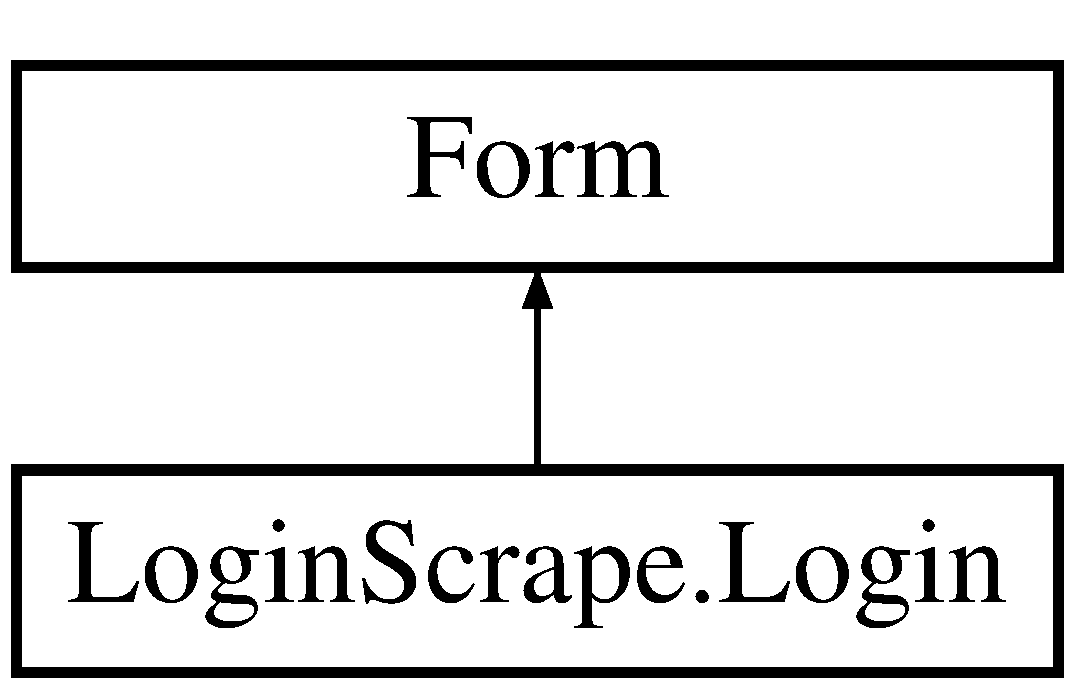
\includegraphics[height=2.000000cm]{class_login_scrape_1_1_login}
\end{center}
\end{figure}
\subsection*{Protected Member Functions}
\begin{DoxyCompactItemize}
\item 
override void \hyperlink{class_login_scrape_1_1_login_a75ef91c856cb125b0b0af2b9af9fb470}{Dispose} (bool disposing)
\begin{DoxyCompactList}\small\item\em Clean up any resources being used. \end{DoxyCompactList}\end{DoxyCompactItemize}
\subsection*{Properties}
\begin{DoxyCompactItemize}
\item 
\hypertarget{class_login_scrape_1_1_login_afb5df674c55555c1d566614f0471a111}{}string {\bfseries Username}\hspace{0.3cm}{\ttfamily  \mbox{[}get\mbox{]}}\label{class_login_scrape_1_1_login_afb5df674c55555c1d566614f0471a111}

\item 
\hypertarget{class_login_scrape_1_1_login_a514c2ba5f09dd7b7c123d3c6639621f8}{}string {\bfseries Password}\hspace{0.3cm}{\ttfamily  \mbox{[}get\mbox{]}}\label{class_login_scrape_1_1_login_a514c2ba5f09dd7b7c123d3c6639621f8}

\end{DoxyCompactItemize}


\subsection{Member Function Documentation}
\hypertarget{class_login_scrape_1_1_login_a75ef91c856cb125b0b0af2b9af9fb470}{}\index{Login\+Scrape\+::\+Login@{Login\+Scrape\+::\+Login}!Dispose@{Dispose}}
\index{Dispose@{Dispose}!Login\+Scrape\+::\+Login@{Login\+Scrape\+::\+Login}}
\subsubsection[{Dispose(bool disposing)}]{\setlength{\rightskip}{0pt plus 5cm}override void Login\+Scrape.\+Login.\+Dispose (
\begin{DoxyParamCaption}
\item[{bool}]{disposing}
\end{DoxyParamCaption}
)\hspace{0.3cm}{\ttfamily [protected]}}\label{class_login_scrape_1_1_login_a75ef91c856cb125b0b0af2b9af9fb470}


Clean up any resources being used. 


\begin{DoxyParams}{Parameters}
{\em disposing} & true if managed resources should be disposed; otherwise, false.\\
\hline
\end{DoxyParams}


The documentation for this class was generated from the following files\+:\begin{DoxyCompactItemize}
\item 
Login.\+cs\item 
Login.\+Designer.\+cs\end{DoxyCompactItemize}

\hypertarget{class_login_scrape_1_1_reddit_karma_scraper}{}\section{Login\+Scrape.\+Reddit\+Karma\+Scraper Class Reference}
\label{class_login_scrape_1_1_reddit_karma_scraper}\index{Login\+Scrape.\+Reddit\+Karma\+Scraper@{Login\+Scrape.\+Reddit\+Karma\+Scraper}}
Inheritance diagram for Login\+Scrape.\+Reddit\+Karma\+Scraper\+:\begin{figure}[H]
\begin{center}
\leavevmode
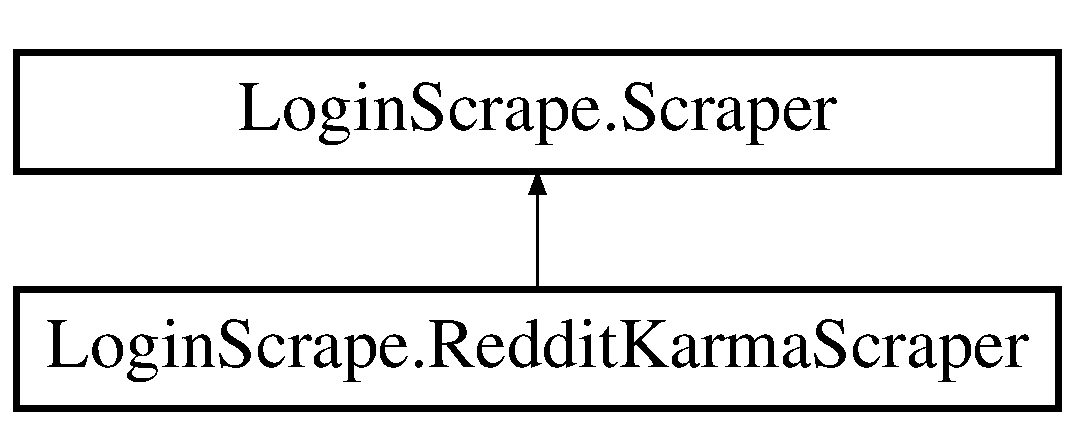
\includegraphics[height=2.000000cm]{class_login_scrape_1_1_reddit_karma_scraper}
\end{center}
\end{figure}
\subsection*{Public Member Functions}
\begin{DoxyCompactItemize}
\item 
\hypertarget{class_login_scrape_1_1_reddit_karma_scraper_a79ebe25ea641c3e2d917074fe617c566}{}{\bfseries Reddit\+Karma\+Scraper} (string username, string password, Text\+Box output\+Control)\label{class_login_scrape_1_1_reddit_karma_scraper_a79ebe25ea641c3e2d917074fe617c566}

\item 
override void \hyperlink{class_login_scrape_1_1_reddit_karma_scraper_add1f029f1c1b7a66c7935bc99ac85df3}{Scrape} ()
\begin{DoxyCompactList}\small\item\em Sets up the scraper state machine and starts the scraping process. \end{DoxyCompactList}\end{DoxyCompactItemize}
\subsection*{Additional Inherited Members}


\subsection{Member Function Documentation}
\hypertarget{class_login_scrape_1_1_reddit_karma_scraper_add1f029f1c1b7a66c7935bc99ac85df3}{}\index{Login\+Scrape\+::\+Reddit\+Karma\+Scraper@{Login\+Scrape\+::\+Reddit\+Karma\+Scraper}!Scrape@{Scrape}}
\index{Scrape@{Scrape}!Login\+Scrape\+::\+Reddit\+Karma\+Scraper@{Login\+Scrape\+::\+Reddit\+Karma\+Scraper}}
\subsubsection[{Scrape()}]{\setlength{\rightskip}{0pt plus 5cm}override void Login\+Scrape.\+Reddit\+Karma\+Scraper.\+Scrape (
\begin{DoxyParamCaption}
{}
\end{DoxyParamCaption}
)\hspace{0.3cm}{\ttfamily [virtual]}}\label{class_login_scrape_1_1_reddit_karma_scraper_add1f029f1c1b7a66c7935bc99ac85df3}


Sets up the scraper state machine and starts the scraping process. 



Implements \hyperlink{class_login_scrape_1_1_scraper_a39769c81c7b10937f7434bc37967f1ac}{Login\+Scrape.\+Scraper}.



The documentation for this class was generated from the following file\+:\begin{DoxyCompactItemize}
\item 
Reddit\+Karma\+Scraper.\+cs\end{DoxyCompactItemize}

\hypertarget{class_login_scrape_1_1_scraper}{}\section{Login\+Scrape.\+Scraper Class Reference}
\label{class_login_scrape_1_1_scraper}\index{Login\+Scrape.\+Scraper@{Login\+Scrape.\+Scraper}}
Inheritance diagram for Login\+Scrape.\+Scraper\+:\begin{figure}[H]
\begin{center}
\leavevmode
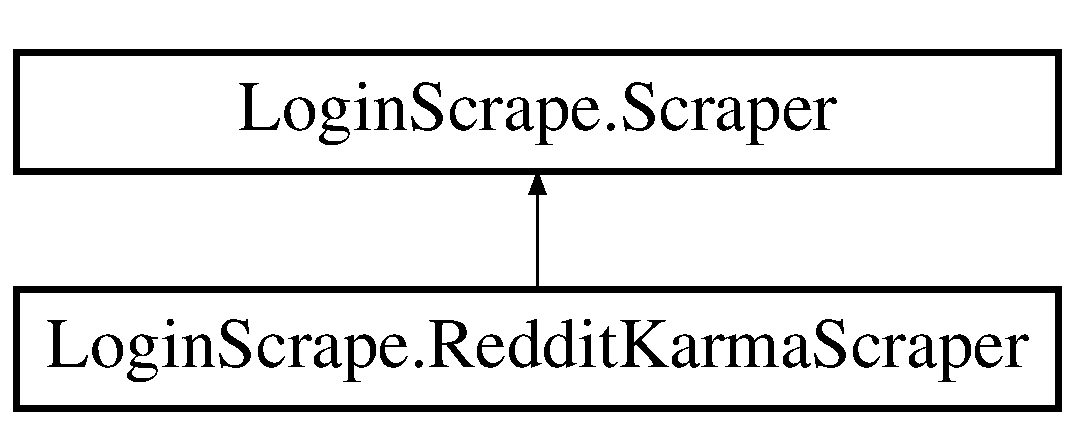
\includegraphics[height=2.000000cm]{class_login_scrape_1_1_scraper}
\end{center}
\end{figure}
\subsection*{Public Member Functions}
\begin{DoxyCompactItemize}
\item 
abstract void \hyperlink{class_login_scrape_1_1_scraper_a39769c81c7b10937f7434bc37967f1ac}{Scrape} ()
\begin{DoxyCompactList}\small\item\em Starts the scraping process. \end{DoxyCompactList}\end{DoxyCompactItemize}
\subsection*{Protected Member Functions}
\begin{DoxyCompactItemize}
\item 
delegate bool \hyperlink{class_login_scrape_1_1_scraper_ae0fba0647c6e6cc40496a7beda2059db}{Scraper\+Step} ()
\begin{DoxyCompactList}\small\item\em This is a function that is called whenever the site being navigated by the scraper finished loading a new page. \end{DoxyCompactList}\item 
void \hyperlink{class_login_scrape_1_1_scraper_a9b55b5146c6ea2c920e86f05be8b55ac}{Add\+Scraper\+Step} (int state, \hyperlink{class_login_scrape_1_1_scraper_ae0fba0647c6e6cc40496a7beda2059db}{Scraper\+Step} fun)
\begin{DoxyCompactList}\small\item\em Registers a function with a scraper state. \end{DoxyCompactList}\item 
void \hyperlink{class_login_scrape_1_1_scraper_a2f6a2da9e29aa031bc9c99895b73a6d2}{Add\+Transition} (int from\+State, int to\+State)
\begin{DoxyCompactList}\small\item\em Registers a scraper state transition. \end{DoxyCompactList}\item 
void \hyperlink{class_login_scrape_1_1_scraper_a101712d2bcbc483cbca2e18a42d14971}{Advance} ()
\begin{DoxyCompactList}\small\item\em If the current state is the error state, it unhooks the scraper from its browser\textquotesingle{}s Document\+Completed event. Otherwise, it performs the function indicated for the current state. The state of the scraper will also be advanced if that function returns true. \end{DoxyCompactList}\item 
void \hyperlink{class_login_scrape_1_1_scraper_a58ba947ea3a7753ad5077e701b84afb0}{Set\+Error\+State} ()
\begin{DoxyCompactList}\small\item\em Sets the scraper to the error state. \end{DoxyCompactList}\end{DoxyCompactItemize}
\subsection*{Protected Attributes}
\begin{DoxyCompactItemize}
\item 
\hypertarget{class_login_scrape_1_1_scraper_a96acb3744f3e89d179e169b4d74e4994}{}Web\+Browser {\bfseries browser}\label{class_login_scrape_1_1_scraper_a96acb3744f3e89d179e169b4d74e4994}

\end{DoxyCompactItemize}
\subsection*{Static Protected Attributes}
\begin{DoxyCompactItemize}
\item 
\hypertarget{class_login_scrape_1_1_scraper_aca4931a8a34120868e56cf2d74689298}{}static int {\bfseries E\+R\+R\+O\+R\+\_\+\+S\+T\+A\+T\+E} = unchecked((int)0xffffffff)\label{class_login_scrape_1_1_scraper_aca4931a8a34120868e56cf2d74689298}

\item 
\hypertarget{class_login_scrape_1_1_scraper_aeba14b6e882a3f186aa9f2947aed6b7f}{}static int {\bfseries S\+T\+A\+R\+T\+\_\+\+S\+T\+A\+T\+E} = unchecked((int)0xfffffffe)\label{class_login_scrape_1_1_scraper_aeba14b6e882a3f186aa9f2947aed6b7f}

\item 
\hypertarget{class_login_scrape_1_1_scraper_addac70144841af5e78fc5f12097b739e}{}static int {\bfseries F\+I\+N\+I\+S\+H\+\_\+\+S\+T\+A\+T\+E} = unchecked((int)0xfffffffd)\label{class_login_scrape_1_1_scraper_addac70144841af5e78fc5f12097b739e}

\end{DoxyCompactItemize}


\subsection{Member Function Documentation}
\hypertarget{class_login_scrape_1_1_scraper_a9b55b5146c6ea2c920e86f05be8b55ac}{}\index{Login\+Scrape\+::\+Scraper@{Login\+Scrape\+::\+Scraper}!Add\+Scraper\+Step@{Add\+Scraper\+Step}}
\index{Add\+Scraper\+Step@{Add\+Scraper\+Step}!Login\+Scrape\+::\+Scraper@{Login\+Scrape\+::\+Scraper}}
\subsubsection[{Add\+Scraper\+Step(int state, Scraper\+Step fun)}]{\setlength{\rightskip}{0pt plus 5cm}void Login\+Scrape.\+Scraper.\+Add\+Scraper\+Step (
\begin{DoxyParamCaption}
\item[{int}]{state, }
\item[{{\bf Scraper\+Step}}]{fun}
\end{DoxyParamCaption}
)\hspace{0.3cm}{\ttfamily [protected]}}\label{class_login_scrape_1_1_scraper_a9b55b5146c6ea2c920e86f05be8b55ac}


Registers a function with a scraper state. 


\begin{DoxyParams}{Parameters}
{\em state} & \\
\hline
{\em fun} & \\
\hline
\end{DoxyParams}
\hypertarget{class_login_scrape_1_1_scraper_a2f6a2da9e29aa031bc9c99895b73a6d2}{}\index{Login\+Scrape\+::\+Scraper@{Login\+Scrape\+::\+Scraper}!Add\+Transition@{Add\+Transition}}
\index{Add\+Transition@{Add\+Transition}!Login\+Scrape\+::\+Scraper@{Login\+Scrape\+::\+Scraper}}
\subsubsection[{Add\+Transition(int from\+State, int to\+State)}]{\setlength{\rightskip}{0pt plus 5cm}void Login\+Scrape.\+Scraper.\+Add\+Transition (
\begin{DoxyParamCaption}
\item[{int}]{from\+State, }
\item[{int}]{to\+State}
\end{DoxyParamCaption}
)\hspace{0.3cm}{\ttfamily [protected]}}\label{class_login_scrape_1_1_scraper_a2f6a2da9e29aa031bc9c99895b73a6d2}


Registers a scraper state transition. 


\begin{DoxyParams}{Parameters}
{\em from\+State} & \\
\hline
{\em to\+State} & \\
\hline
\end{DoxyParams}
\hypertarget{class_login_scrape_1_1_scraper_a101712d2bcbc483cbca2e18a42d14971}{}\index{Login\+Scrape\+::\+Scraper@{Login\+Scrape\+::\+Scraper}!Advance@{Advance}}
\index{Advance@{Advance}!Login\+Scrape\+::\+Scraper@{Login\+Scrape\+::\+Scraper}}
\subsubsection[{Advance()}]{\setlength{\rightskip}{0pt plus 5cm}void Login\+Scrape.\+Scraper.\+Advance (
\begin{DoxyParamCaption}
{}
\end{DoxyParamCaption}
)\hspace{0.3cm}{\ttfamily [protected]}}\label{class_login_scrape_1_1_scraper_a101712d2bcbc483cbca2e18a42d14971}


If the current state is the error state, it unhooks the scraper from its browser\textquotesingle{}s Document\+Completed event. Otherwise, it performs the function indicated for the current state. The state of the scraper will also be advanced if that function returns true. 

\hypertarget{class_login_scrape_1_1_scraper_a39769c81c7b10937f7434bc37967f1ac}{}\index{Login\+Scrape\+::\+Scraper@{Login\+Scrape\+::\+Scraper}!Scrape@{Scrape}}
\index{Scrape@{Scrape}!Login\+Scrape\+::\+Scraper@{Login\+Scrape\+::\+Scraper}}
\subsubsection[{Scrape()}]{\setlength{\rightskip}{0pt plus 5cm}abstract void Login\+Scrape.\+Scraper.\+Scrape (
\begin{DoxyParamCaption}
{}
\end{DoxyParamCaption}
)\hspace{0.3cm}{\ttfamily [pure virtual]}}\label{class_login_scrape_1_1_scraper_a39769c81c7b10937f7434bc37967f1ac}


Starts the scraping process. 



Implemented in \hyperlink{class_login_scrape_1_1_reddit_karma_scraper_add1f029f1c1b7a66c7935bc99ac85df3}{Login\+Scrape.\+Reddit\+Karma\+Scraper}.

\hypertarget{class_login_scrape_1_1_scraper_ae0fba0647c6e6cc40496a7beda2059db}{}\index{Login\+Scrape\+::\+Scraper@{Login\+Scrape\+::\+Scraper}!Scraper\+Step@{Scraper\+Step}}
\index{Scraper\+Step@{Scraper\+Step}!Login\+Scrape\+::\+Scraper@{Login\+Scrape\+::\+Scraper}}
\subsubsection[{Scraper\+Step()}]{\setlength{\rightskip}{0pt plus 5cm}delegate bool Login\+Scrape.\+Scraper.\+Scraper\+Step (
\begin{DoxyParamCaption}
{}
\end{DoxyParamCaption}
)\hspace{0.3cm}{\ttfamily [protected]}}\label{class_login_scrape_1_1_scraper_ae0fba0647c6e6cc40496a7beda2059db}


This is a function that is called whenever the site being navigated by the scraper finished loading a new page. 

\begin{DoxyReturn}{Returns}
True if the scraper should advance to the next state, i.\+e. if another page has been requested. Return false to keep the scraper from automatically moving to the next state, i.\+e. if loading more dynamically generated data from the same page, or if an error condition has been encountered.
\end{DoxyReturn}
\hypertarget{class_login_scrape_1_1_scraper_a58ba947ea3a7753ad5077e701b84afb0}{}\index{Login\+Scrape\+::\+Scraper@{Login\+Scrape\+::\+Scraper}!Set\+Error\+State@{Set\+Error\+State}}
\index{Set\+Error\+State@{Set\+Error\+State}!Login\+Scrape\+::\+Scraper@{Login\+Scrape\+::\+Scraper}}
\subsubsection[{Set\+Error\+State()}]{\setlength{\rightskip}{0pt plus 5cm}void Login\+Scrape.\+Scraper.\+Set\+Error\+State (
\begin{DoxyParamCaption}
{}
\end{DoxyParamCaption}
)\hspace{0.3cm}{\ttfamily [protected]}}\label{class_login_scrape_1_1_scraper_a58ba947ea3a7753ad5077e701b84afb0}


Sets the scraper to the error state. 



The documentation for this class was generated from the following file\+:\begin{DoxyCompactItemize}
\item 
Scraper.\+cs\end{DoxyCompactItemize}

%--- End generated contents ---

% Index
\backmatter
\newpage
\phantomsection
\clearemptydoublepage
\addcontentsline{toc}{chapter}{Index}
\printindex

\end{document}
